%%%%%%%%%%%%%%%%%%%%%%%%%%%%%%%%%%%
%This is the LaTeX ARTICLE template for RSC journals
%Copyright The Royal Society of Chemistry 2016
%%%%%%%%%%%%%%%%%%%%%%%%%%%%%%%%%%%

\documentclass[twoside,twocolumn,9pt]{article}
\usepackage{extsizes}
\usepackage[super,sort&compress,comma]{natbib} 
\usepackage[version=3]{mhchem}
\usepackage[left=1.5cm, right=1.5cm, top=1.785cm, bottom=2.0cm]{geometry}
\usepackage{balance}
\usepackage{mathptmx}
\usepackage{sectsty}
\usepackage{graphicx} 
\usepackage{lastpage}
\usepackage[format=plain,justification=justified,singlelinecheck=false,font={stretch=1.125,small,sf},labelfont=bf,labelsep=space]{caption}
\usepackage{float}
\usepackage{fancyhdr}
\usepackage{fnpos}
\usepackage[english]{babel}
\addto{\captionsenglish}{%
  \renewcommand{\refname}{Notes and references}
}
\usepackage{array}
\usepackage{droidsans}
\usepackage{charter}
\usepackage[T1]{fontenc}
\usepackage[usenames,dvipsnames]{xcolor}
\usepackage{setspace}
\usepackage[compact]{titlesec}
\usepackage{hyperref}
%%%Please don't disable any packages in the preamble, as this may cause the template to display incorrectly.%%%


\usepackage{epstopdf}%This line makes .eps figures into .pdf - please comment out if not required.

\definecolor{cream}{RGB}{222,217,201}

\begin{document}

\pagestyle{fancy}
\thispagestyle{plain}
\fancypagestyle{plain}{
%%%HEADER%%%
\renewcommand{\headrulewidth}{0pt}
}
%%%END OF HEADER%%%

%%%PAGE SETUP - Please do not change any commands within this section%%%
\makeFNbottom
\makeatletter
\renewcommand\LARGE{\@setfontsize\LARGE{15pt}{17}}
\renewcommand\Large{\@setfontsize\Large{12pt}{14}}
\renewcommand\large{\@setfontsize\large{10pt}{12}}
\renewcommand\footnotesize{\@setfontsize\footnotesize{7pt}{10}}
\makeatother

\renewcommand{\thefootnote}{\fnsymbol{footnote}}
\renewcommand\footnoterule{\vspace*{1pt}% 
\color{cream}\hrule width 3.5in height 0.4pt \color{black}\vspace*{5pt}} 
\setcounter{secnumdepth}{5}

\makeatletter 
\renewcommand\@biblabel[1]{#1}            
\renewcommand\@makefntext[1]% 
{\noindent\makebox[0pt][r]{\@thefnmark\,}#1}
\makeatother 
\renewcommand{\figurename}{\small{Fig.}~}
\sectionfont{\sffamily\Large}
\subsectionfont{\normalsize}
\subsubsectionfont{\bf}
\setstretch{1.125} %In particular, please do not alter this line.
\setlength{\skip\footins}{0.8cm}
\setlength{\footnotesep}{0.25cm}
\setlength{\jot}{10pt}
\titlespacing*{\section}{0pt}{4pt}{4pt}
\titlespacing*{\subsection}{0pt}{15pt}{1pt}
\setlength{\parskip}{1em}
%%%END OF PAGE SETUP%%%

%%%FOOTER%%%
\pagestyle{fancy} % Turn on the style
\fancyhf{} % Start with clearing everything in the header and footer
% Set the right side of the footer to be the page number
\fancyfoot[R]{\thepage}

% Redefine plain style, which is used for titlepage and chapter beginnings
% From https://tex.stackexchange.com/a/30230/828
\fancypagestyle{plain}{%
    \renewcommand{\headrulewidth}{0pt}%
    \fancyhf{}%
    \fancyfoot[R]{\thepage}%
}

\renewcommand{\headrulewidth}{0pt} 
\renewcommand{\footrulewidth}{0pt}
\setlength{\arrayrulewidth}{1pt}
\setlength{\columnsep}{6.5mm}
\setlength\bibsep{1pt}
%%%END OF FOOTER%%%

%%%FIGURE SETUP - please do not change any commands within this section%%%
\makeatletter 
\newlength{\figrulesep} 
\setlength{\figrulesep}{0.5\textfloatsep} 

\newcommand{\topfigrule}{\vspace*{-1pt}% 
\noindent{\color{cream}\rule[-\figrulesep]{\columnwidth}{1.5pt}} }

\newcommand{\botfigrule}{\vspace*{-2pt}% 
\noindent{\color{cream}\rule[\figrulesep]{\columnwidth}{1.5pt}} }

\newcommand{\dblfigrule}{\vspace*{-1pt}% 
\noindent{\color{cream}\rule[-\figrulesep]{\textwidth}{1.5pt}} }

\makeatother
%%%END OF FIGURE SETUP%%%

%%%TITLE, AUTHORS AND ABSTRACT%%%
%\twocolumn[
\begin{@twocolumnfalse}
\vspace{1em}
\sffamily

\hrule
\vspace{2em}
\noindent\centering\LARGE{\textbf{Classifying Images of Fashion Items using Deep CNN}} \\%Article title goes here instead of the text "This is the title"
\vspace{1em}
\noindent\large{Cheng Xi Tsou, Ningyu Chen, and Tim Betancur}\\%Author names go here instead of "Full name", etc.
\vspace{2em}
\hrule
\vspace{1em}
% \noindent\normalsize{The abstract should be a single paragraph which summarises the content of the article. Any references in the abstract should be written out in full \textit{e.g.}\ [Surname \textit{et al., Journal Title}, 2000, \textbf{35}, 3523].} \\%The abstrast goes here instead of the text "The abstract should be..."

\end{@twocolumnfalse}
\vspace{0.6cm}
%]

%%%END OF TITLE, AUTHORS AND ABSTRACT%%%

%%%FONT SETUP - please do not change any commands within this section
\renewcommand*\rmdefault{bch}\normalfont\upshape
\rmfamily
\section*{}
\vspace{-1cm}


%%%FOOTNOTES%%%




%%%END OF FOOTNOTES%%%

%%%MAIN TEXT%%%%
\section{Introduction}
In $2020$, around $30\%$ of the total fashion retail sales in the US were through e-commerce. Countless new products were introduced during each season of the year. Listing new products into respective categories by human power could be time consuming and error-prone. We decided to solve this problem by building a classifier through a deep convolutional neural network that can efficiently and accurately classify images of fashion items. Our final model is able to classify images of fashion items with a 0.923 accuracy into 8 article types. 

\section{Data}

The data we used to train our network were 80 by 60 RGB images from Kaggle\cite{Kaggle}. The dataset came with 44,000 images labeled with 136 different article types and other basic descriptors of each image. After examining our dataset, we found an extreme imbalance between the classes, so we picked the classes that had at least 1700 samples and capped each class at 2500 samples, which resulted in 8 classes. We ended up with about 17,000 images with a 80-10-10 split between training, validation, and testing. Initially, we resized the images to 28 by 28 on grayscale but later we procured two more sets of data with dimensions 28x28 RGB and 80x60 RGB. For data preprocessing, we scaled each data value to be in the range of [0, 1] and changed our labels into categorical one-hot encoding. 

\begin{figure}[h]
\centering
  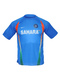
\includegraphics[height=3cm]{images/1163}
  \caption{A 80x60 sample image}
  \label{fgr:example}
\end{figure}

\section{Experiments and Results}
We started our experiments with a baseline model from Keras' Simple MNIST convnet \cite{Keras} implementation as a reference and progressively introduced more complexity. This allowed us to learn whether a certain hyperparameter tuning was effective. The baseline model was a simple CNN with the following structure: (3, 3, 16) Conv, (2, 2) MaxPool, (3, 3, 64) Conv, (2, 2) MaxPool, (8) Dense. This model had a reasonable performance achieving 0.835 accuracy on the test set. The results indicated which classes were harder to classify and what the model was lacking.


\begin{table}[h]
\small
  \caption{\ Evaluation of baseline model on testing data}
  \label{tbl:example1}
  \begin{tabular*}{0.48\textwidth}{@{\extracolsep{\fill}}lll}
    \hline
    Class name & f1-score & support \\
    \hline
    Sports Shoes & 0.807107 & 203 \\
    Kurtas & 0.885714 & 244 \\
    Tops & 0.933687 & 188 \\
    Handbags & 0.771144 & 194 \\
    Watches & 0.993603 & 235 \\
    Shirts & 0.854167 & 233 \\
    Tshirts & 0.842520 & 263 \\
    Casual Shoes & 0.983333 & 180 \\
    Accuracy & 0.882759 & N/A \\
    Macro avg & 0.883909 & 1740 \\
    Weighted avg & 0.882869 & 1740 \\
    \hline
  \end{tabular*}
\end{table}

\subsection{Experiment 1}

In this experiment, we continuously added one layer, a Conv layer or dense layer, to our baseline model until the accuracy in the validation set did not improve anymore. Each succeeding model has one more layer than the previous. The images had low resolutions(28 x 28), so we did not introduce more pooling layers. We expanded the two stacks of Conv. layers by duplicating existing Conv layers. We added paddings to each Conv layer to maintain the input dimensions. It helped to elongate the network, which enabled us to add more Conv layers. We expanded the stacks of Conv layers and dense layers alternatively. We added more Conv layers when the model needed to capture more captures. We added more dense layers when the model needed more parameters to enhance its classification power. We stopped when the model was no longer improving and its computational time was too long. The validation accuracy of each model was compared, and we selected the model, exp1\_10, with the highest validation accuracy. Model exp1\_10 had 6 Conv layers equally divided between the stacks and three dense layers.

\begin{table}[h]
\small
  \caption{\ The image above displays the performance of each model.}
  \label{tbl:example1}
  \begin{tabular*}{0.48\textwidth}{@{\extracolsep{\fill}}llll}
    \hline
    Model name & Accuracy & Validation Accuracy & Acc Diff\\
    \hline
    exp1\_10 & 0.944862 & 0.900383 & 0.044\\
    exp1\_5 & 0.938192 & 0.897190 & 0.041\\
    exp1\_7 & 0.949262 & 0.896552 & 0.053\\
    exp1\_11 & 0.938689 & 0.895913 & 0.043\\
    exp1\_6 & 0.934644 & 0.894636 & 0.040\\
    exp1\_4 & 0.928683 & 0.893997 & 0.035\\
    exp1\_8 & 0.956713 & 0.892720 & 0.064\\
    exp1\_9 & 0.934076 & 0.885696 & 0.048\\
    exp1\_1 & 0.920380 & 0.884419 & 0.036\\
    exp1\_3 & 0.927689 & 0.884419 & 0.043\\
    exp1\_2 & 0.933579 & 0.883780 & 0.050\\
    \hline
  \end{tabular*}
\end{table}

\noindent Model exp1\_5 underperformed by around 0.3\%. Its architecture was less complex than model exp\_1\_10; it was nearly two times faster. However, our goal for this experiment was to choose the model with the best generalization ability. Then we would apply simplification and regularization to the selected model in the later experiments. 


\subsection{Experiment 2}

In this experiment, we tried to improve the performance of model exp1\_10 by increasing the deeper Conv layers’ kernel sizes. The convention of building a CNN architecture is to gradually increase the kernel size to reduce the feature space width to capture high-level information. The pattern of kernel sizes used for the second stack of Conv layers are listed as follow: (5x5) (5x5) (5x5), (3x3) (3x3) (5x5), (3x3)(5x5)(3x3), (5x5)(3x3)(3x3), and substituted (7x7) for (5x5). There are 8 different patterns and thus 8 models. According to the results, these alterations did not improve the generalization ability of model exp1\_10, but in fact, they caused more overfitting on the testing set. Generally, larger kernel size should combat overfitting as it helps to capture generic features. However, the output dimensions of the first max pooling layer was (13x13). Therefore, we were unknowingly converting Conv layers to fully connected layers by using relatively big kernel sizes, which undermined the generalization ability of CNN and thus caused overfitting. As a result, we will proceed with exp1\_10 as our current best model.

\begin{table}[h]
\small
  \caption{\ The table displays the performance of each model.
Please note: a model with higher label number is more complex due to layer additions}
  \label{tbl:example1}
  \begin{tabular*}{0.48\textwidth}{@{\extracolsep{\fill}}llll}
    \hline
    Model name & Accuracy & Validation Accuracy & Acc Diff\\
    \hline
    exp2\_10\_6 & 0.959 & 0.898 & 0.061\\
    exp2\_10\_1 & 0.953 & 0.897 & 0.056\\
    exp2\_10\_5 & 0.948 & 0.895 & 0.053\\
    exp2\_10\_7  & 0.941 & 0.893 & 0.047\\
    exp2\_10\_8  & 0.960 & 0.892 & 0.068\\
    exp2\_10\_4  & 0.958 & 0.891 & 0.068\\
    exp2\_10\_9  & 0.927 & 0.887 & 0.040\\
    \hline
  \end{tabular*}
\end{table}

\subsection{Experiment 3}

In this experiment, the goal was to combat our issue of overfitting. The best model we have so far yielded a training accuracy of 0.944 and a validation accuracy of 0.9. Our goal is to reduce the difference between the two so that the model is less overfit on the data we have trained it on and able to be generalized for new inputs. The strategies that we have tried to employ are adding Dropout layers in the Dense layers, adding Dropout layers with low dropout rates in the convolutional layers, adding L2 regularization to the Dense layer’s kernel weights, and data augmentation. 

\noindent Our first model exp3\_10\_2 had two Dropout layers with dropout rate at 0.3 in the Dense layer, then we added Dropout layers with dropout rates at 0.2 to our convolutional layers for our model exp3\_10\_3. The results showed that both approaches still resulted in slight overfitting. After tuning the dropout rates in all layers, the results favored the model exp3\_10\_1 with two dropout layers with dropout rate of 0.5 in the dense layers. We hypothesize that this was because our image contained important low level features so any kind of dropout will cause the model to be less generalizable. We also tested a model exp3\_10\_4 with data augmentation with horizontal flips, rotations, and random offsets but the results showed a drop in training and validation accuracy. 

\noindent Finally, we decided to try to simplify the model as we thought that the excessive number of layers caused our model not to generalize well. After removing a convolutional layer from each stack of convolutional layers and having two Dropout layers with dropout rates of 0.5 in the dense layer, we were able to finalize a model exp3\_10\_8 that had a training accuracy of 0.9145 and validation accuracy of 0.8978. Compared to other models in this experiment, exp3\_10\_8 converged much faster so it was less prone to overfitting. Comparing this exp3\_10\_8 with our best model from experiment exp1\_10, the two models had a similar validation accuracy but exp3\_10\_8 is better generalized.

\begin{figure}[h]
\centering
  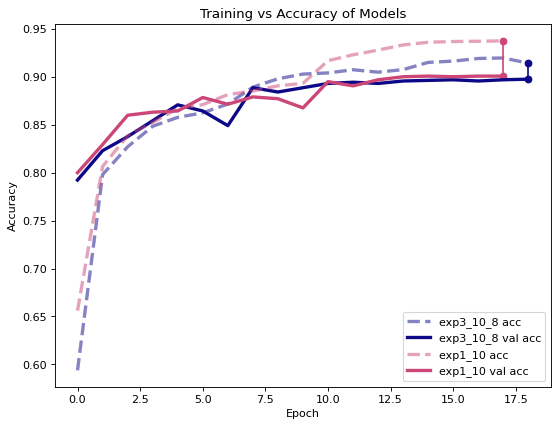
\includegraphics[height=6.5cm]{images/exp3}
  \caption{Comparing the current best model with previous best model}
  \label{fgr:example}
\end{figure}

\begin{table}[h]
\small
  \caption{\ The table displays the performance of each model.}
  \label{tbl:example1}
  \begin{tabular*}{0.48\textwidth}{@{\extracolsep{\fill}}llll}
    \hline
    Model name & Accuracy & Validation Accuracy & Acc Diff\\
    \hline
    exp3\_10\_7 & 0.934 & 0.898 & 0.036\\
    exp3\_10\_8 & 0.914 & 0.898 & 0.017\\
    exp3\_10\_2 & 0.939 & 0.895 & 0.044\\
    exp3\_10\_3 & 0.940 & 0.895 & 0.045\\
    exp3\_10\_1 & 0.924 & 0.891 & 0.033\\
    exp3\_10\_5 & 0.910 & 0.889 & 0.021\\
    exp3\_10\_6 & 0.907 & 0.889 & 0.019\\
    exp3\_10\_4 & 0.841 & 0.844 & -0.003\\
    \hline
  \end{tabular*}
\end{table}

\subsection{Experiment 4}
In this experiment, we wanted to try to change the width of the model so that our model is able to extract more features and find more patterns to classify our fashion items. Although we had hypothesized that our model was overfitting because it was too complex, we wanted to test our hypothesis. The strategies we will employ in this experiment are tuning the number of filters in the convolutional layers and tuning the number of units in the dense layer. 

\noindent First, we wanted to see if the model needed to extract more features by using 64 and 128 as our number of filters in our model exp4\_10\_3\_1 but this resulted in an overfit. Then, we decided to lower our number of filters for models exp4\_10\_3\_2 and exp4\_10\_3\_3. While this did not cause the model to overfit, the model’s validation accuracy went down. In the following models exp4\_10\_3\_4 to exp4\_10\_3\_7, we wanted to test if our model needed more classification power by increasing the units in our dense layers and experimented with different numbers of filters in our convolutional layers. The result was still overfitting which aligns with our original hypothesis that our model did not need to be more complex. We will keep the previous best model and proceed with exp3\_10\_3 in experiment 5.

\begin{table}[h]
\small
  \caption{\ The table displays the performance of each model.}
  \label{tbl:example1}
  \begin{tabular*}{0.48\textwidth}{@{\extracolsep{\fill}}llll}
    \hline
    Model name & Accuracy & Validation Accuracy & Acc Diff\\
    \hline
    exp4\_10\_8\_5 & 0.926 & 0.900 & 0.026\\
    exp4\_10\_8\_4 & 0.924 & 0.898 & 0.026\\
    exp4\_10\_8\_1 & 0.956 & 0.895 & 0.061\\
    exp4\_10\_8\_7 & 0.928 & 0.892 & 0.004\\
    exp4\_10\_8\_6 & 0.930 & 0.891 & 0.004\\
    exp4\_10\_8\_2 & 0.898 & 0.887 & 0.011\\
    exp4\_10\_8\_3 & 0.909 & 0.882 & 0.027\\
    \hline
  \end{tabular*}
\end{table}

\subsection{Experiment 5}
We were unable to increase the model’s validation accuracy by hyperparameter tuning. So in this experiment we changed the dataset. The original dataset is 80x60x3, but we chose to use grayscale for faster training time as we thought colors wouldn’t be relevant and would confuse the model. However upon revision, we hypothesized that RGB would matter as different article types may have a set color palette that designers use. In this experiment, we will test and refine our model using image dimensions of 28x28x3 and 80x60x3. 

\noindent First, we trained our model on the input dimensions 28x28x3. This resulted in an increase of validation accuracy to a new high of 0.9138. Then, we increased the number of units in our dense layer for models exp5\_10\_8\_2, exp5\_10\_8\_3 as we thought with 3 channels, there would be more classification power needed. However, the validation accuracy did not improve. We then trained our model exp5\_10\_8\_4 with increased units in the Dense layers on our data with dimensions 80x60x3 and further increased our validation accuracy. However, the training time took a long time as the number of parameters for the model was 10 million. In model exp5\_10\_8\_5, we added in a group of convolutional layers with max pooling so the data is downsampled and added a Dropout layer with dropout rate of 0.1 after each group of convolutions to combat overfitting. This reduced the parameters of our model to 2 million and achieved a final validation accuracy of 0.928. 


\begin{table}[h]
\small
  \caption{\ The table displays the performance of each model.}
  \label{tbl:example1}
  \begin{tabular*}{0.48\textwidth}{@{\extracolsep{\fill}}llll}
    \hline
    Model name & Accuracy & Validation Accuracy & Acc Diff\\
    \hline
    exp5\_10\_8\_5 & 0.961 & 0.928 & 0.032\\
    exp5\_10\_8\_4  & 0.959 & 0.921 & 0.037\\
    exp5\_10\_8\_3  & 0.944 & 0.917 & 0.027\\
    exp5\_10\_8\_1  & 0.935 & 0.914 & 0.021\\
    exp5\_10\_8\_2  & 0.940 & 0.914 & 0.026\\
    \hline
  \end{tabular*}
\end{table}

\begin{table}[h]
\small
  \caption{\ Composition of exp5\_10\_8\_5}
  \label{tbl:example1}
  \begin{tabular*}{0.48\textwidth}{@{\extracolsep{\fill}}llll}
    \hline
    Layer (type) & Output Shape & Param \# \\
    \hline
    Conv         & (80, 60, 16) & 448      \\
    Conv         & (80, 60, 16) & 2320     \\
    Max Pool     & (40, 30, 16) & 0        \\
    Dropout      & (40, 30, 16) & 0        \\
    Conv         & (40, 30, 32) & 4640     \\
    Conv         & (40, 30, 32) & 9248     \\
    Max Pool     & (20, 15, 32) & 0        \\
    Dropout      & (20, 15, 32) & 0        \\
    Conv         & (20, 15, 64) & 18494    \\
    Conv         & (20, 15, 64) & 36928    \\
    Max Pool     & (10, 7, 64)  & 0        \\
    Dropout      & (10, 7, 64)  & 0        \\
    Flatten      & (4480)       & 0        \\
    Dense        & (512)        & 2294272  \\
    Dropout      & (512)        & 0        \\
    Dense        & (512)        & 262656   \\
    Dropout      & (512)        & 0        \\
    Dense        & (512)        & 262656   \\
    Dense        & (8)          & 4104     \\
    \hline
  \end{tabular*}
\end{table}

\noindent Comparing the best models of each input dimension, we found that the validation accuracy steadily increased. For the final model, we chose to use exp5\_10\_8\_5 with input dimensions of 80x60x3. An evaluation of our final model on testing data showed an accuracy of 0.913. This was much better than our baseline model which had an accuracy of 0.835. 

\begin{figure}[h]
\centering
  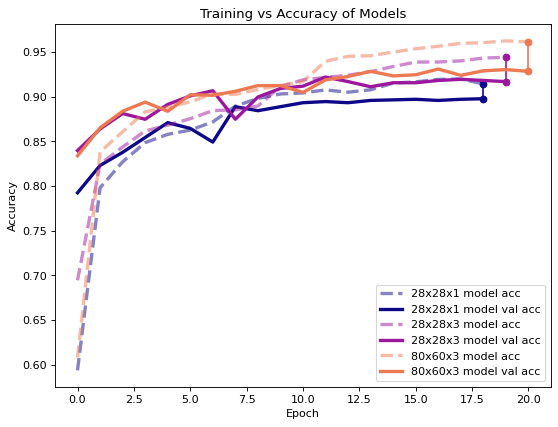
\includegraphics[height=6.8cm]{images/exp5}
  \caption{Comparing the best models of each input dimension}
  \label{fgr:example}
\end{figure}

\noindent Looking at a confusion matrix (see Figure 4 below) of predictions on our final model, we found that the model did very well for classes with more distinct shapes, and poorly on classes that were similar in shape. Most notably, the pairs of classes that had the highest proportion of mislabeling as one another were Shirts and Tops, and Kurtas and T-shirts.

\begin{figure*}
\centering
  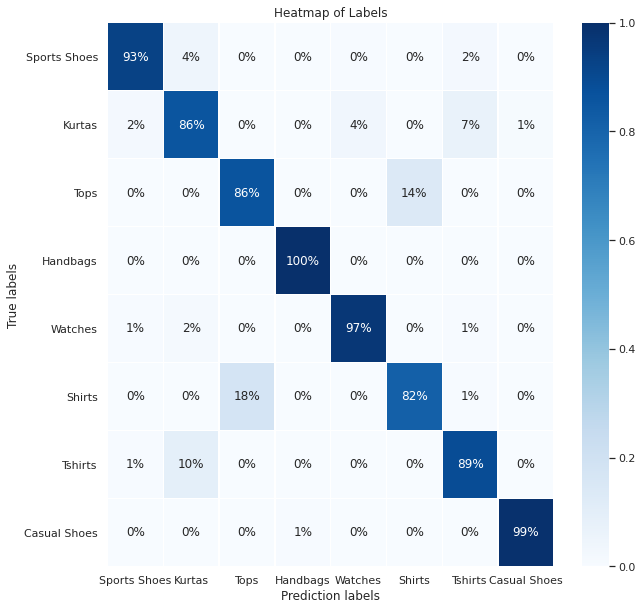
\includegraphics[height=6.8cm]{images/matrix}
  \caption{Comparing the best models of each input dimension}
  \label{fgr:example2col}
\end{figure*}

\section{Retrospective}
We learned the conventions of building a CNN architecture and fine-tuning hyperparameters to obtain the best model. We saw the importance of the quality of the input images. The performance of the models increased the greatest when input images were colored instead of grayscale. We had limited computation resources on Google Colab, so we traded the resolutions and colors of input images for training efficiency. Experiment 5 demonstrated that the colors enhanced the models' classification ability. So better performance could be achieved if we did not down sample the images.

\section{Appendix}

First, go to our github to download the neccessary files. The github link is found here\cite{github}. Download all the files inside the "files" folder. There should be 4 zips. Download the notebook  "FashionCNN\_final.ipynb" in the "notebook" folder to run the final model for our project. For a more detailed walkthrough of our project including all experiment and data preprocessing, download the notebook "FashionCNN\_detailed.ipynb". Instructions to run the detailed version will be found in the detailed notebook.

\subsection{Running FashionCNN\_final.ipynb}
After unzipping the zip files in the "files" folder, there were be four folders. "assets" will contain assets of the final model. "variables" will contain variables of the final model. "model\_histories" will contain the model histories of all our experiments and models. "saved\_files" will contain all our preprocessed data. There are instructions in the detailed notebook on how to reproduce all the data, but due to the run time, we will be loading all our variables and data in this notebook. 

\noindent Please change the paths to each folder in the notebook to wherever you placed these folders. If you are running the notebook on Google Colab, you can upload the zips to your Drive and unzip these folders in the Colab. Make sure to run the appropriate shell commands given in the notebook if you want to mount your Drive. Before running the code, make sure you have the following libraries: Numpy, Pandas, Seaborn, Matplotlib, scikit-learn, TensorFlow
Follow the instructions given in the notebook and you should be able to reproduce our model, the evaluation results, and the confusion matrix. 


%%%END OF MAIN TEXT%%%

%The \balance command can be used to balance the columns on the final page if desired. It should be placed anywhere within the first column of the last page.

% \balance

%If notes are included in your references you can change the title from 'References' to 'Notes and references' using the following command:
%\renewcommand\refname{Notes and references}

%%%REFERENCES%%%
\bibliography{rsc} %You need to replace "rsc" on this line with the name of your .bib file
\bibliographystyle{rsc} %the RSC's .bst file

\end{document}
